\chapter{Results}\label{chapter_results}

This Chapter is concerned with the presentation of the results of a practical
application of the algorithms implemented in
Chapter~\ref{chapter_implementation} as well as and the performance of the
overall integrated system.

\section{Template Matching Tracker}
This Section presents with a qualitative analysis of both the adaptive and
non-adaptive Template Matching Trackers proposed in
Section~\ref{theoretical_framework_template_matching_trackers}. 

Both trackers were applied to the famous Hamburg taxi sequence \cite{} as an initial
test of their applicability to the Motion Tracking Problem.

The Template Trackers below were run for a threshold of 0.8.

\subsection{Simple Template Matching}
The initial template used is the shown by the rectangular region around the car
in the first frame. The images shown correspond to almost equally spaced
samples of the 40 frame taxi sequence.

\begin{figure}\label{fig:simple_template_tracking}
    \makebox[\linewidth][c]{
    \begin{tabular}{cccc}
        \subfloat{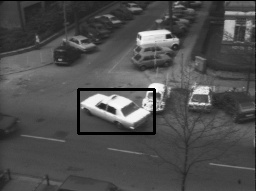
\includegraphics[width = 1.5in]{figures/results/simple_template_tracker/taxi_sequence/1.jpg}} &
        \subfloat{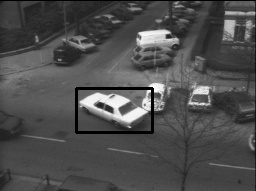
\includegraphics[width = 1.5in]{figures/results/simple_template_tracker/taxi_sequence/2.jpg}} &
        \subfloat{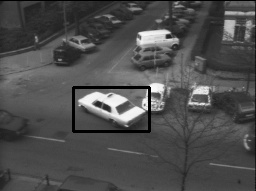
\includegraphics[width = 1.5in]{figures/results/simple_template_tracker/taxi_sequence/3.jpg}} &
        \subfloat{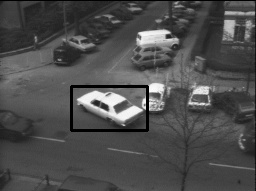
\includegraphics[width = 1.5in]{figures/results/simple_template_tracker/taxi_sequence/4.jpg}} \\

        \subfloat{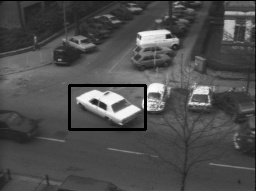
\includegraphics[width = 1.5in]{figures/results/simple_template_tracker/taxi_sequence/5.jpg}} &
        \subfloat{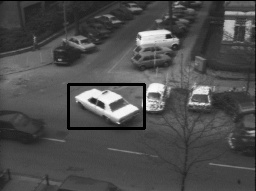
\includegraphics[width = 1.5in]{figures/results/simple_template_tracker/taxi_sequence/6.jpg}} &
        \subfloat{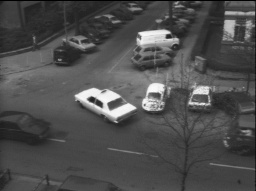
\includegraphics[width = 1.5in]{figures/results/simple_template_tracker/taxi_sequence/7.jpg}} &
        \subfloat{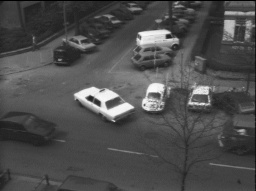
\includegraphics[width = 1.5in]{figures/results/simple_template_tracker/taxi_sequence/8.jpg}} \\
       
        \subfloat{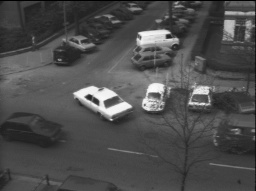
\includegraphics[width = 1.5in]{figures/results/simple_template_tracker/taxi_sequence/9.jpg}} &
        \subfloat{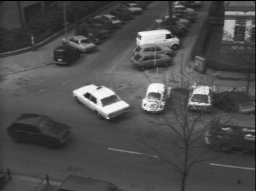
\includegraphics[width = 1.5in]{figures/results/simple_template_tracker/taxi_sequence/10.jpg}} &
        \subfloat{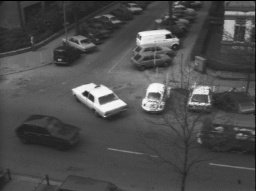
\includegraphics[width = 1.5in]{figures/results/simple_template_tracker/taxi_sequence/11.jpg}} &
        \subfloat{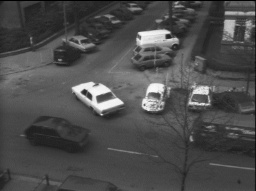
\includegraphics[width = 1.5in]{figures/results/simple_template_tracker/taxi_sequence/12.jpg}} \\
       
        \subfloat{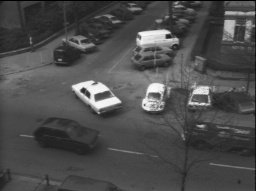
\includegraphics[width = 1.5in]{figures/results/simple_template_tracker/taxi_sequence/13.jpg}} &
        \subfloat{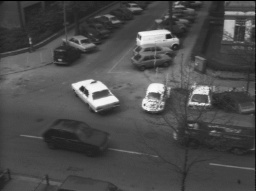
\includegraphics[width = 1.5in]{figures/results/simple_template_tracker/taxi_sequence/14.jpg}} &
        \subfloat{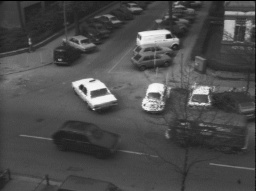
\includegraphics[width = 1.5in]{figures/results/simple_template_tracker/taxi_sequence/15.jpg}} &
        \subfloat{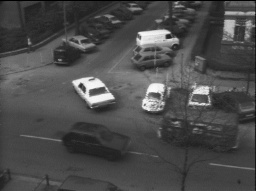
\includegraphics[width = 1.5in]{figures/results/simple_template_tracker/taxi_sequence/16.jpg}} \\   

        \end{tabular}}
    \caption{Simple Template Tracking Hamburg Sequence}
\end{figure}

In Figure~\ref{fig:simple_template_tracking} it can be seen that the Simple Template Matching Algorithm manages to track
the car up until frame 12 of the sequence, beyond which the rotation of the car
drives the Sum of Square Differences similarity measure between the initial template chosen in
$\mathbf{f}_0$ and the region of interest in $\mathbf{f}_{12}$ below the
threshold of 0.8.

Lowering the detection threshold allows the tracker to follow the
car for a larger amount of frames, however this is not a solution to the problem
as the tracker becomes more susceptible to noise, and is certainly not a good
model for robustness across different sequences.

An idea to get around the changing template, is the implementation of an
Adaptive Template Matching Algorithm.

\subsection{Adaptive Template Matching}
As described in Section~\ref{theoretical_framework_adaptive_tm}, the assumption
that an object maintains the same appearance is only valid for an interval of
$K$ frames. Beyond this interval, $\mathbf{f}_{k}$ is sufficiently different
from $\mathbf{f}_{k+K}$ for our similarity measure to fall below the similarity
threshold, $\tau$.

The idea behind this variant of Template Tracker is that by updating the
template which we are trying to match before the we traverse more than
$K$-frames.

The sequence in Figure~\ref{fig:adaptive_template_tracking} is generated by
updating the template every frame, the located object in frame,
$\mathbf{f}_{k-1}$. becomes the template for $\mathbf{f}_k$.

\begin{figure}     
    \makebox[\linewidth][c]{
    \begin{tabular}{cccc}
        \subfloat{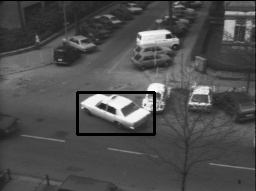
\includegraphics[width = 1.5in]{figures/results/adaptive_template_tracker/taxi_sequence/1.jpg}} &
        \subfloat{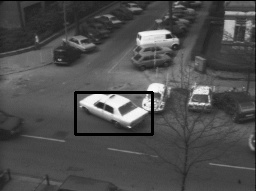
\includegraphics[width = 1.5in]{figures/results/adaptive_template_tracker/taxi_sequence/2.jpg}} &
        \subfloat{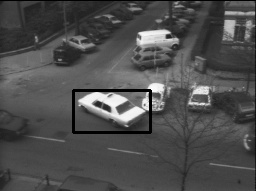
\includegraphics[width = 1.5in]{figures/results/adaptive_template_tracker/taxi_sequence/3.jpg}} &
        \subfloat{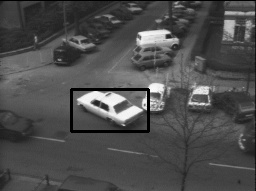
\includegraphics[width = 1.5in]{figures/results/adaptive_template_tracker/taxi_sequence/4.jpg}} \\

        \subfloat{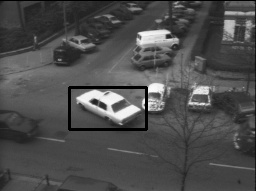
\includegraphics[width = 1.5in]{figures/results/adaptive_template_tracker/taxi_sequence/5.jpg}} &
        \subfloat{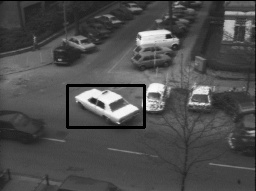
\includegraphics[width = 1.5in]{figures/results/adaptive_template_tracker/taxi_sequence/6.jpg}} &
        \subfloat{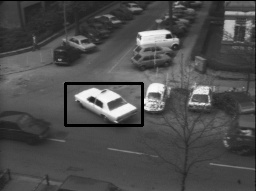
\includegraphics[width = 1.5in]{figures/results/adaptive_template_tracker/taxi_sequence/7.jpg}} &
        \subfloat{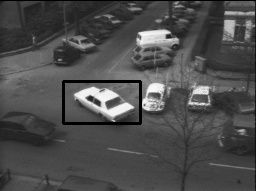
\includegraphics[width = 1.5in]{figures/results/adaptive_template_tracker/taxi_sequence/8.jpg}} \\
       
        \subfloat{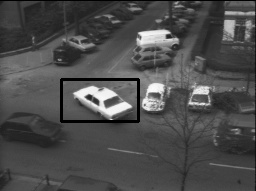
\includegraphics[width = 1.5in]{figures/results/adaptive_template_tracker/taxi_sequence/9.jpg}} &
        \subfloat{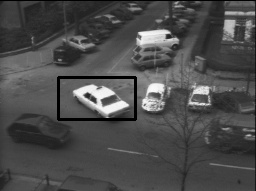
\includegraphics[width = 1.5in]{figures/results/adaptive_template_tracker/taxi_sequence/10.jpg}} &
        \subfloat{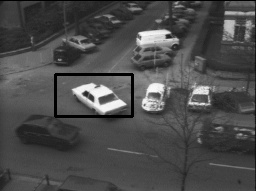
\includegraphics[width = 1.5in]{figures/results/adaptive_template_tracker/taxi_sequence/11.jpg}} &
        \subfloat{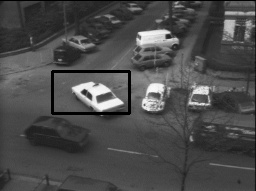
\includegraphics[width = 1.5in]{figures/results/adaptive_template_tracker/taxi_sequence/12.jpg}} \\
       
        \subfloat{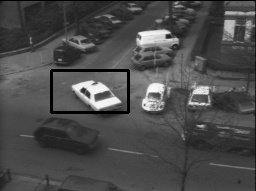
\includegraphics[width = 1.5in]{figures/results/adaptive_template_tracker/taxi_sequence/13.jpg}} &
        \subfloat{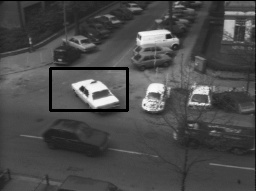
\includegraphics[width = 1.5in]{figures/results/adaptive_template_tracker/taxi_sequence/14.jpg}} &
        \subfloat{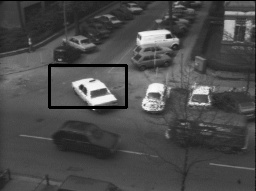
\includegraphics[width = 1.5in]{figures/results/adaptive_template_tracker/taxi_sequence/15.jpg}} &
        \subfloat{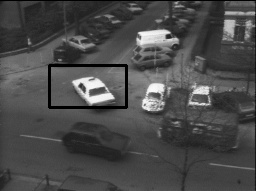
\includegraphics[width = 1.5in]{figures/results/adaptive_template_tracker/taxi_sequence/16.jpg}} \\   

        \end{tabular}}
    \caption{Adaptive Template Tracking Hamburg Sequence\label{fig:adaptive_template_tracking}
 }
\end{figure}

From Figure~\ref{fig:adaptive_template_tracking} it shows that the Adaptive
Template Tracker manages to locate the car within a bounding box in each frame
of the sequence. It should however be noted that there is a noticeable ``drift'' in
the localisation. 
This is due to the fact that the template selected does not solely 


\section{Colour Co-occurrence Histogram}

\section{Mean Shift Tracking}
This Section deals with the qualitative analysis of the Mean Shift Tracker
implemented in Section~\ref{implementation_mean_shift_tracker}. The analysis is
broken down into a set of experiments,

There are generally three parameters that a user can vary when using the mean
shift tracker. 
\begin{itemize}
    \item $\epsilon$ - step size bounding maximum mean shift vector magnitude
    \item $m$ - bin count of histograms
    \item $(h_x,h_y)$ - kernel dimensions and positioning around or on object
\end{itemize}
We subsequently assess the performance of the Mean Shift Tracker implementation
for varying parameters $\epsilon$ and $m$ for the sequence in order to see the
effect their on tracker performance, the goal being to select reasonable values
for the two parameters to asses the general practical performance of the Mean
Shift Tracker. 

We perform this assessment in a series of experiments, each of which is based on an image
sequence that exhibits one or more of the challenges to motion tracking outlined
in Section~\ref{literature_review_challenges}. 
 
The image sequences presented are taken from the datasets provided by the VOT2017
challenge \cite{VOT_TPAMI}.

\subsection{Experiment 1: Fish}
This sequence is one in which there are several fish, of which a distinctly yellow fish is
tracked. The challenges to motion tracking that arise in this image sequence are the following.
\begin{itemize}
    \item Occlusion (complete)
    \item Scaling 
    \item Ego motion (slight) 
\end{itemize}

The relevant sub-sequences of interest are documented below:

\subsubsection{Partial Occlusion}\label{mean_shift_partial_occlusion}

\begin{figure}     
    \makebox[\linewidth][c]{
    \begin{tabular}{cccc}
        \subfloat{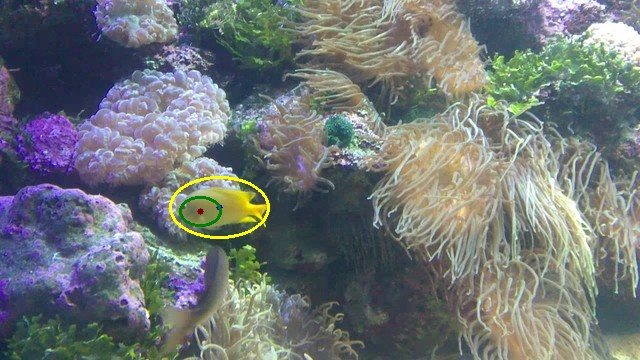
\includegraphics[width = 1.5in]{figures/results/mean_shift_tracker/fish3/occlusion/1.jpg}} &
        \subfloat{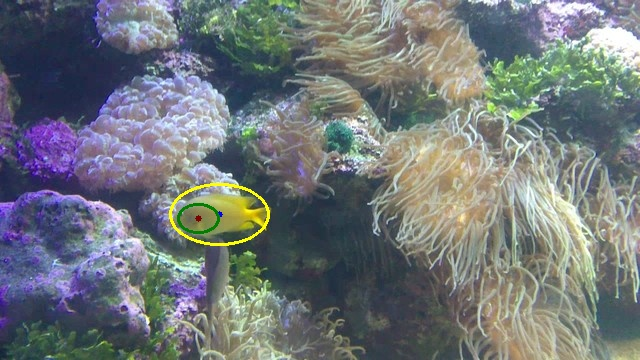
\includegraphics[width = 1.5in]{figures/results/mean_shift_tracker/fish3/occlusion/2.jpg}} &
        \subfloat{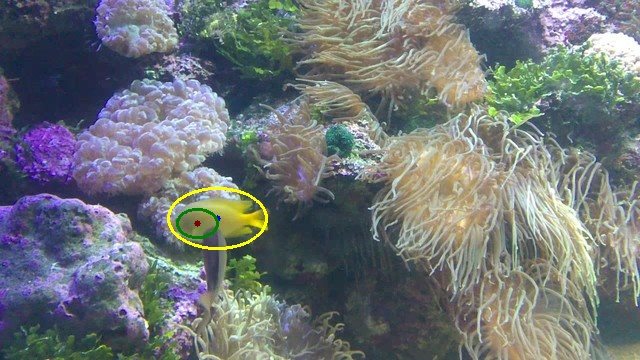
\includegraphics[width = 1.5in]{figures/results/mean_shift_tracker/fish3/occlusion/3.jpg}} &
        \subfloat{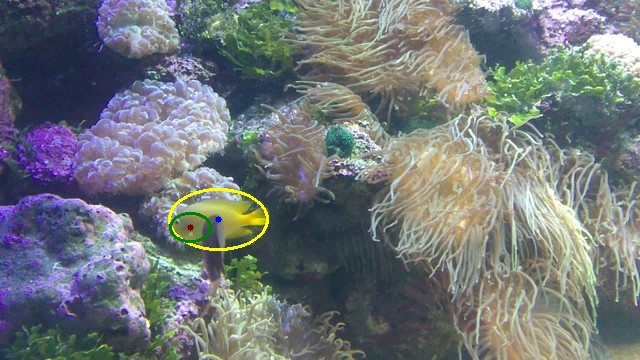
\includegraphics[width = 1.5in]{figures/results/mean_shift_tracker/fish3/occlusion/4.jpg}} \\

        \subfloat{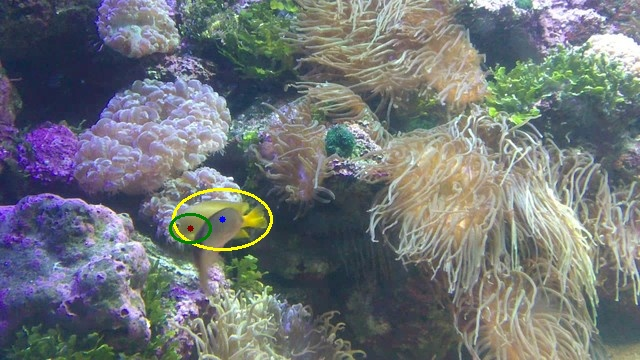
\includegraphics[width = 1.5in]{figures/results/mean_shift_tracker/fish3/occlusion/5.jpg}} &
        \subfloat{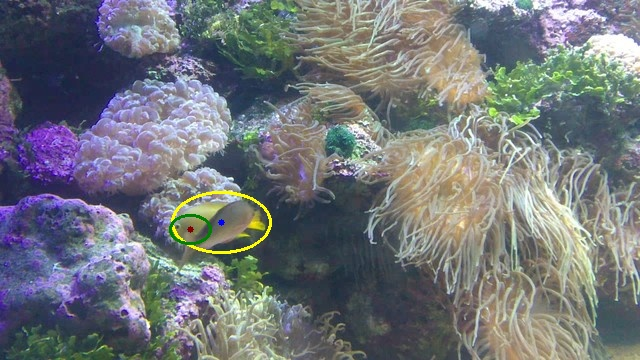
\includegraphics[width = 1.5in]{figures/results/mean_shift_tracker/fish3/occlusion/6.jpg}} &
        \subfloat{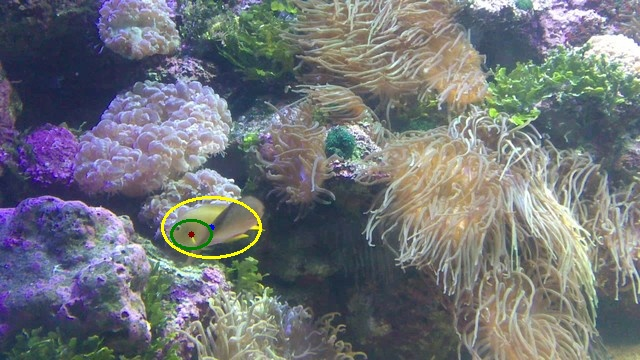
\includegraphics[width = 1.5in]{figures/results/mean_shift_tracker/fish3/occlusion/7.jpg}} &
        \subfloat{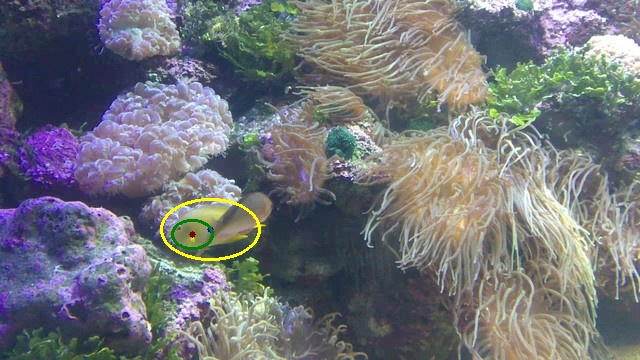
\includegraphics[width = 1.5in]{figures/results/mean_shift_tracker/fish3/occlusion/8.jpg}} \\
       
        \subfloat{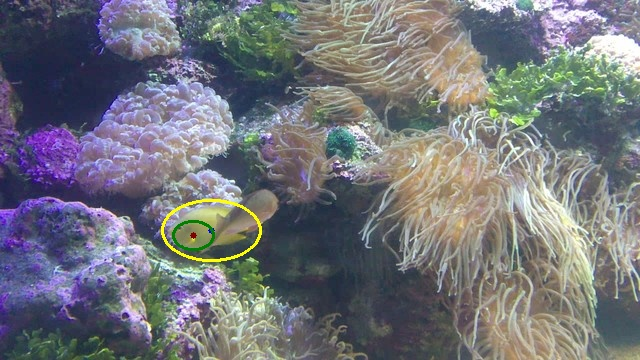
\includegraphics[width = 1.5in]{figures/results/mean_shift_tracker/fish3/occlusion/9.jpg}} &
        \subfloat{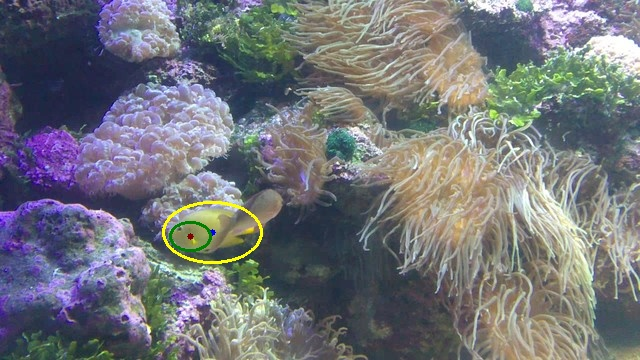
\includegraphics[width = 1.5in]{figures/results/mean_shift_tracker/fish3/occlusion/10.jpg}} &
        \subfloat{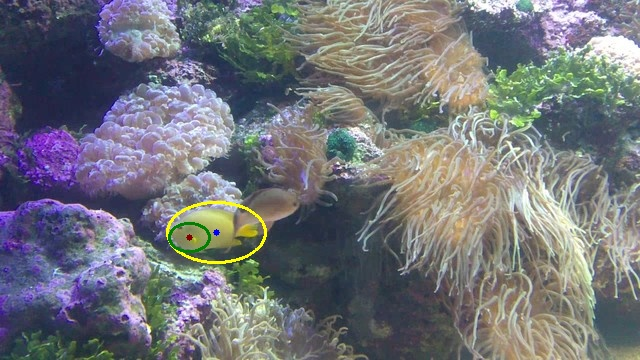
\includegraphics[width = 1.5in]{figures/results/mean_shift_tracker/fish3/occlusion/11.jpg}} &
        \subfloat{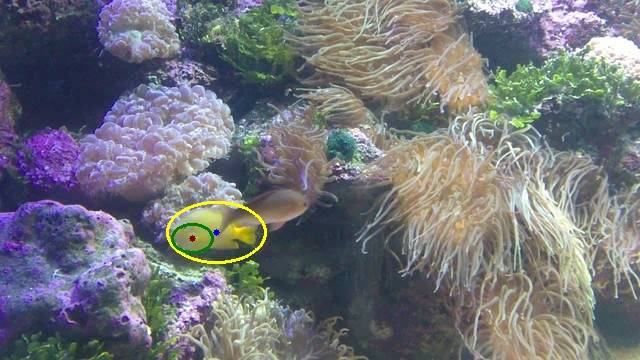
\includegraphics[width = 1.5in]{figures/results/mean_shift_tracker/fish3/occlusion/12.jpg}} \\
       
        \subfloat{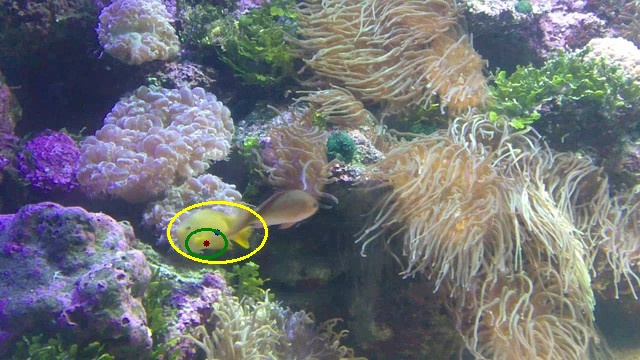
\includegraphics[width = 1.5in]{figures/results/mean_shift_tracker/fish3/occlusion/13.jpg}} &
        \subfloat{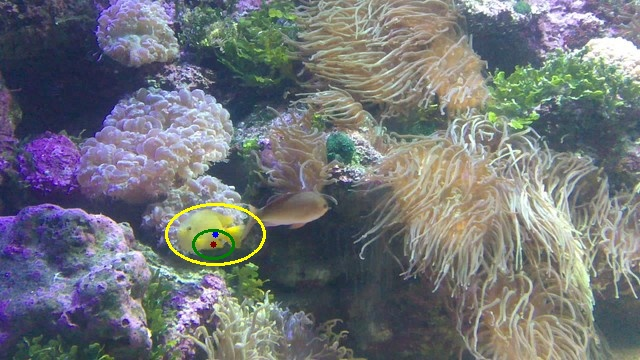
\includegraphics[width = 1.5in]{figures/results/mean_shift_tracker/fish3/occlusion/14.jpg}} &
        \subfloat{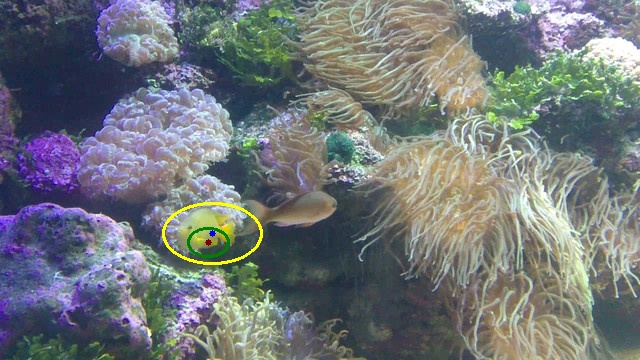
\includegraphics[width = 1.5in]{figures/results/mean_shift_tracker/fish3/occlusion/15.jpg}} &
        \subfloat{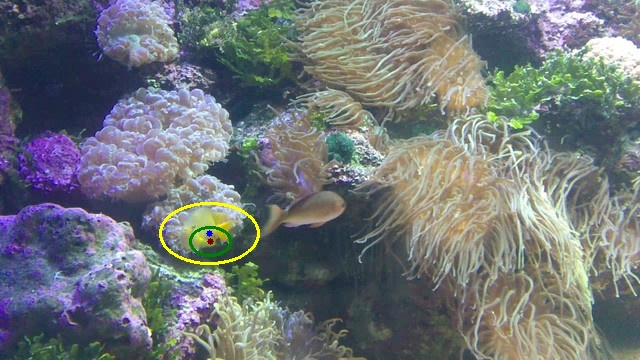
\includegraphics[width = 1.5in]{figures/results/mean_shift_tracker/fish3/occlusion/16.jpg}} \\   

        \end{tabular}}
    \caption{Challenge: Partial Occlusion\label{fig:mean_shift_partial_occlusion}
 }
\end{figure}


\subsubsection{Changing Orientation}

\begin{figure}     
    \makebox[\linewidth][c]{
    \begin{tabular}{cccc}
        \subfloat{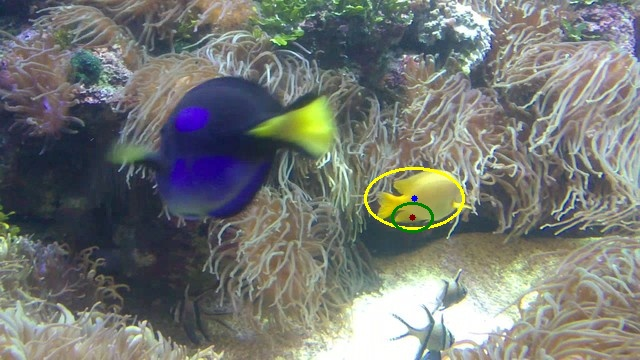
\includegraphics[width = 1.5in]{figures/results/mean_shift_tracker/fish3/orientation/1.jpg}} &
        \subfloat{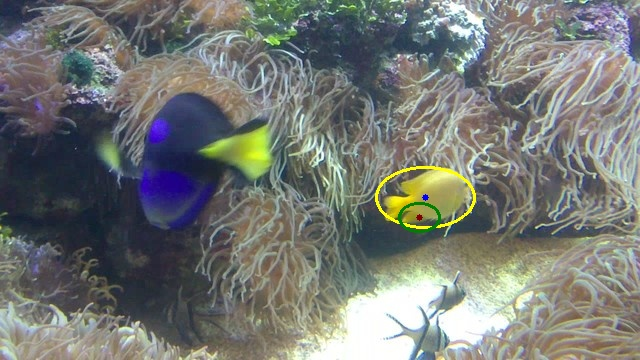
\includegraphics[width = 1.5in]{figures/results/mean_shift_tracker/fish3/orientation/2.jpg}} &
        \subfloat{\includegraphics[width = 1.5in]{figures/results/mean_shift_tracker/fish3/orientation/3.jpg}} &
        \subfloat{\includegraphics[width = 1.5in]{figures/results/mean_shift_tracker/fish3/orientation/4.jpg}} \\

        \subfloat{\includegraphics[width = 1.5in]{figures/results/mean_shift_tracker/fish3/orientation/5.jpg}} &
        \subfloat{\includegraphics[width = 1.5in]{figures/results/mean_shift_tracker/fish3/orientation/6.jpg}} &
        \subfloat{\includegraphics[width = 1.5in]{figures/results/mean_shift_tracker/fish3/orientation/7.jpg}} &
        \subfloat{\includegraphics[width = 1.5in]{figures/results/mean_shift_tracker/fish3/orientation/8.jpg}} \\
       
        \subfloat{\includegraphics[width = 1.5in]{figures/results/mean_shift_tracker/fish3/orientation/9.jpg}} &
        \subfloat{\includegraphics[width = 1.5in]{figures/results/mean_shift_tracker/fish3/orientation/10.jpg}} &
        \subfloat{\includegraphics[width = 1.5in]{figures/results/mean_shift_tracker/fish3/orientation/11.jpg}} &
        \subfloat{\includegraphics[width = 1.5in]{figures/results/mean_shift_tracker/fish3/orientation/12.jpg}} \\
       
        \subfloat{\includegraphics[width = 1.5in]{figures/results/mean_shift_tracker/fish3/orientation/13.jpg}} &
        \subfloat{\includegraphics[width = 1.5in]{figures/results/mean_shift_tracker/fish3/orientation/14.jpg}} &
        \subfloat{\includegraphics[width = 1.5in]{figures/results/mean_shift_tracker/fish3/orientation/15.jpg}} &
        \subfloat{\includegraphics[width = 1.5in]{figures/results/mean_shift_tracker/fish3/orientation/16.jpg}} \\   

        \end{tabular}}
    \caption{Challenge: Changing Orientation\label{fig:mean_shift_orientation}
 }
\end{figure}

\subsection{Experiment 2: Girl}
This sequence is one of a Girl in a park riding around on a scooter. She is
wearing a distinctive colourful outfit relative to the rest of the moving objects in the
scene, which consist mostly other humans.
The relevant challenges presented in this scene are:
\begin{itemize}
    \item Occlusion (complete)
    \item Scaling 
    \item Ego motion (slight) 
\end{itemize}

\subsubsection{Complete Occlusion}
The relevant subsequence exhibiting occlusion ranges from $\mathbf{f}_{97}$ to
$\mathbf{f}_{127}$ and is presented in Figure~\ref{fig:mean_shift_complete_occlusion}.

\begin{figure}    
    \makebox[\linewidth][c]{
    \begin{tabular}{cccc}
        \subfloat{\includegraphics[width = 1.5in]{figures/results/mean_shift_tracker/girl/occlusion/1.jpg}} &
        \subfloat{\includegraphics[width = 1.5in]{figures/results/mean_shift_tracker/girl/occlusion/2.jpg}} &
        \subfloat{\includegraphics[width = 1.5in]{figures/results/mean_shift_tracker/girl/occlusion/3.jpg}} &
        \subfloat{\includegraphics[width = 1.5in]{figures/results/mean_shift_tracker/girl/occlusion/4.jpg}} \\

        \subfloat{\includegraphics[width = 1.5in]{figures/results/mean_shift_tracker/girl/occlusion/5.jpg}} &
        \subfloat{\includegraphics[width = 1.5in]{figures/results/mean_shift_tracker/girl/occlusion/6.jpg}} &
        \subfloat{\includegraphics[width = 1.5in]{figures/results/mean_shift_tracker/girl/occlusion/7.jpg}} &
        \subfloat{\includegraphics[width = 1.5in]{figures/results/mean_shift_tracker/girl/occlusion/8.jpg}} \\
       
        \subfloat{\includegraphics[width = 1.5in]{figures/results/mean_shift_tracker/girl/occlusion/9.jpg}} &
        \subfloat{\includegraphics[width = 1.5in]{figures/results/mean_shift_tracker/girl/occlusion/10.jpg}} &
        \subfloat{\includegraphics[width = 1.5in]{figures/results/mean_shift_tracker/girl/occlusion/11.jpg}} &
        \subfloat{\includegraphics[width = 1.5in]{figures/results/mean_shift_tracker/girl/occlusion/12.jpg}} \\
       
        \subfloat{\includegraphics[width = 1.5in]{figures/results/mean_shift_tracker/girl/occlusion/13.jpg}} &
        \subfloat{\includegraphics[width = 1.5in]{figures/results/mean_shift_tracker/girl/occlusion/14.jpg}} &
        \subfloat{\includegraphics[width = 1.5in]{figures/results/mean_shift_tracker/girl/occlusion/15.jpg}} &
        \subfloat{\includegraphics[width = 1.5in]{figures/results/mean_shift_tracker/girl/occlusion/16.jpg}} \\   

        \end{tabular}
    }
    \caption{Challenge: Complete Occlusion\label{fig:mean_shift_complete_occlusion}}
\end{figure}

\subsubsection{Scaling}

\begin{figure} 
    \makebox[\linewidth][c]{
    \begin{tabular}{cccc}
        \subfloat{\includegraphics[width = 1.5in]{figures/results/mean_shift_tracker/girl/scale/1.jpg}} &
        \subfloat{\includegraphics[width = 1.5in]{figures/results/mean_shift_tracker/girl/scale/2.jpg}} &
        \subfloat{\includegraphics[width = 1.5in]{figures/results/mean_shift_tracker/girl/scale/3.jpg}} &
        \subfloat{\includegraphics[width = 1.5in]{figures/results/mean_shift_tracker/girl/scale/4.jpg}} \\

        \subfloat{\includegraphics[width = 1.5in]{figures/results/mean_shift_tracker/girl/scale/5.jpg}} &
        \subfloat{\includegraphics[width = 1.5in]{figures/results/mean_shift_tracker/girl/scale/6.jpg}} &
        \subfloat{\includegraphics[width = 1.5in]{figures/results/mean_shift_tracker/girl/scale/7.jpg}} &
        \subfloat{\includegraphics[width = 1.5in]{figures/results/mean_shift_tracker/girl/scale/8.jpg}} \\
       
        \subfloat{\includegraphics[width = 1.5in]{figures/results/mean_shift_tracker/girl/scale/9.jpg}} &
        \subfloat{\includegraphics[width = 1.5in]{figures/results/mean_shift_tracker/girl/scale/10.jpg}} &
        \subfloat{\includegraphics[width = 1.5in]{figures/results/mean_shift_tracker/girl/scale/11.jpg}} &
        \subfloat{\includegraphics[width = 1.5in]{figures/results/mean_shift_tracker/girl/scale/12.jpg}} \\
       
        \subfloat{\includegraphics[width = 1.5in]{figures/results/mean_shift_tracker/girl/scale/13.jpg}} &
        \subfloat{\includegraphics[width = 1.5in]{figures/results/mean_shift_tracker/girl/scale/14.jpg}} &
        \subfloat{\includegraphics[width = 1.5in]{figures/results/mean_shift_tracker/girl/scale/15.jpg}} &
        \subfloat{\includegraphics[width = 1.5in]{figures/results/mean_shift_tracker/girl/scale/16.jpg}} \\   
    \end{tabular}}
    \caption{Challenge: Scale Change\label{fig:mean_shift_girl_scale}}
\end{figure}


\subsection{Experiment 3: Ants}
This image sequence is of multiple ants in motion within a Petri dish.

The challenges presented by this sequence are the following:
\begin{itemize}
    \item Target Speed
    \item Track Overlap
\end{itemize}

\subsubsection{Target Speed}\label{mean_shift_target_speed}
The relevant subsequence ranges from $\mathbf{f}_{202}$ to $\mathbf{f}_{250}$
in the original sequence.
In Figure~\ref{fig:mean_shift_ant_speed}, $\mathbf{F}_{13}$ to $\mathbf{F}_{16}$
highlight this issue, as can be seen by the Green Kernel failing to track the
Ant for the due to its relatively large inter-frame displacement.

\begin{figure}
    \makebox[\linewidth][c]{
    \begin{tabular}{cccc}
        \subfloat{\includegraphics[width = 1.5in]{figures/results/mean_shift_tracker/ants/speed/1.jpg}} &
        \subfloat{\includegraphics[width = 1.5in]{figures/results/mean_shift_tracker/ants/speed/2.jpg}} &
        \subfloat{\includegraphics[width = 1.5in]{figures/results/mean_shift_tracker/ants/speed/3.jpg}} &
        \subfloat{\includegraphics[width = 1.5in]{figures/results/mean_shift_tracker/ants/speed/4.jpg}} \\

        \subfloat{\includegraphics[width = 1.5in]{figures/results/mean_shift_tracker/ants/speed/5.jpg}} &
        \subfloat{\includegraphics[width = 1.5in]{figures/results/mean_shift_tracker/ants/speed/6.jpg}} &
        \subfloat{\includegraphics[width = 1.5in]{figures/results/mean_shift_tracker/ants/speed/7.jpg}} &
        \subfloat{\includegraphics[width = 1.5in]{figures/results/mean_shift_tracker/ants/speed/8.jpg}} \\
       
        \subfloat{\includegraphics[width = 1.5in]{figures/results/mean_shift_tracker/ants/speed/9.jpg}} &
        \subfloat{\includegraphics[width = 1.5in]{figures/results/mean_shift_tracker/ants/speed/10.jpg}} &
        \subfloat{\includegraphics[width = 1.5in]{figures/results/mean_shift_tracker/ants/speed/11.jpg}} &
        \subfloat{\includegraphics[width = 1.5in]{figures/results/mean_shift_tracker/ants/speed/12.jpg}} \\
       
        \subfloat{\includegraphics[width = 1.5in]{figures/results/mean_shift_tracker/ants/speed/13.jpg}} &
        \subfloat{\includegraphics[width = 1.5in]{figures/results/mean_shift_tracker/ants/speed/14.jpg}} &
        \subfloat{\includegraphics[width = 1.5in]{figures/results/mean_shift_tracker/ants/speed/15.jpg}} &
        \subfloat{\includegraphics[width = 1.5in]{figures/results/mean_shift_tracker/ants/speed/16.jpg}} \\   
    \end{tabular}}
    \caption{Challenge: Target Speed\label{fig:mean_shift_ant_speed}}
\end{figure}

As the displacement of an Object between $\mathbf{f}_k$ and $\mathbf{f}_{k+1}$ 
increases in magnitude, less of the Object lies within the dimensions
$(h_x,h_y)$ of the Kernel that we initialise at it's last known pixel location
$\mathbf{c_0}$ in $\mathbf{f}_k$. In terms of the mean shift tracking algorithm this simply
results in a larger mean shift vector, $\vec{m}$.

As shown in Experiment~\ref{results_varying_epsilon}, The Mean Shift Tracker's
parameter $\epsilon$ - which limits the allowed magnitude of $\vec{m}$ between
$\mathbf{f}_{k}$ and $\mathbf{f}_{k+1}$ - can increase the tracker's tolerance
to challenges such as Object speed and occlusion, at the
cost of increased track ``jitter''. 

However Figure~\ref{fig:mean_shift_ant_speed} highlights the extreme case in
which none of the object in  

It is important to clarify in the case of the Ant sequence in particular, the speed of the
object, but the sampling rate, $f_s$ used to obtain the sequence. If a higher
sampling rate were used, would mean higher redundancy between frames with
smaller displacements. So lazy solution could be provide the same sequence
sampled at a higher $f_s$.

Thinking further, there may be situation in which the available technology is
constrained by factors such as budget, size etc. In such situations, we would
still like to be able to track our object of interest. 
A possible solution could be to augment the basic Mean Shift Algorithm with
other forms of more information possibly from other tracking methodologies highlighted in
Figure\ref{fig:motion_tracking_taxonomy}. 

\subsubsection{Track Overlap}
In Figure~\ref{fig:mean_shift_ant_speed}, $\mathbf{F}_5$ to $\mathbf{F}_{11}$
highlight this challenge. We have two ants coming within close proximity of
each other, we can see that the yellow kernel switches to track the second Ant
after the crossing of their tracks within the sequence. Let us refer to the
original ant as $A_0$ and the second ant as $A_1$. 

It is important at this point to highlight the differences between this case of
track overlap, and that detailed in Section~\ref{mean_shift_partial_occlusion},
in which, despite the tracks for the yellow fish and grey fish overlapping
entirely, the tracker remains remains unaffected.
The answer lies within the feature space our tracker is based on. Within the RGB colour space,
the yellow and grey fish are largely distinct. Hence the tracker will not be
drawn to the grey fish as it exits the Yellow Kernel.

In this case, the are two objects within the Yellow Kernel that are practically
indistinguishable within our chose feature space. one ant exits the Kernel, there exists
no gradient within the domain of the similarity function to draw the tracker away.

With $A_0$ and $A_1$ close to each other, The fact that $A_0$ moves with a high
velocity, means that the inter-frame displacement of $A_0$ between
$\mathbf{f}_k$ and $\mathbf{f}_{k+1}$ is easily be large enough to place $A_1$
closer to $A_0$ in $\mathbf{f}_{k+1}$, which makes the mean shift iteration
likely to pick $A_1$ as the target location in $\mathbf{f}_{k+1}$


